\algnewcommand{\LineComment}[1]{\State \(\triangleright\) #1}
% New definitions
\algnewcommand\algorithmicswitch{\textbf{switch}}
\algnewcommand\algorithmiccase{\textbf{case}}
\algnewcommand\algorithmicassert{\text{assert}}
\algnewcommand\Assert[1]{\State \algorithmicassert(#1)}%
% New "environments"
\algdef{SE}[SWITCH]{Switch}{EndSwitch}[1]{\algorithmicswitch\ #1\ \algorithmicdo}{\algorithmicend\ \algorithmicswitch}%
\algdef{SE}[CASE]{Case}{EndCase}[1]{\algorithmiccase\ #1}{\algorithmicend\ \algorithmiccase}%
\algtext*{EndSwitch}%
\algtext*{EndCase}%

% \graphicspath{{Figures/Multi/P2/}{./}} 

\chapter{Simultaneous Multiple Quantile Estimation}
\label{ch: multi_quant}

\graphicspath{{Figures/Multi/}{./}} 

The previously introduced methods estimate only a single quantile. For applications which need multiple quantiles, these methods are not sufficient.\marginpar{This opening phrase is still not very good.}
In this chapter we introduce the problem of simultaneous multi-quantile estimation and two related methods. The structure is organised as follow:

Section~\ref{sec: multi_intro} introduces the multi-quantile estimation for streaming data, followed by a discussion on the basic ideas to approach this problem. The next two sections will show how it is solved by methods focusing on different aspects.

Section~\ref{sec: multi_shiftQ} shows the \textit{shiftQ} algorithm for simultaneous quantile estimation by implementing an idea similar to SGD.

Section~\ref{sec: multi_{p2}} shows the \textit{$P^2$} algorithm that solves the problem in a different way.

% Section~\ref{sec: multi_discussion} compares and contrasts the two methods, the discussion about the problem and our conclusion.

\section{The problem and opportunity of multi-quantile estimation}
\label{sec: multi_intro}

In real life implementations, quantile estimation usually does not focus on a single quantile value. For example, a common request is to show the median (the $0.5$-quantile) of the distribution, and at the same time show the outlier boundaries at ends of the distribution, like the $0.1$- and $0.9$- quantiles. It is also likely that multiple quantile estimates are required for a data distribution analysis.

\begin{figure}[h]
    \centering
	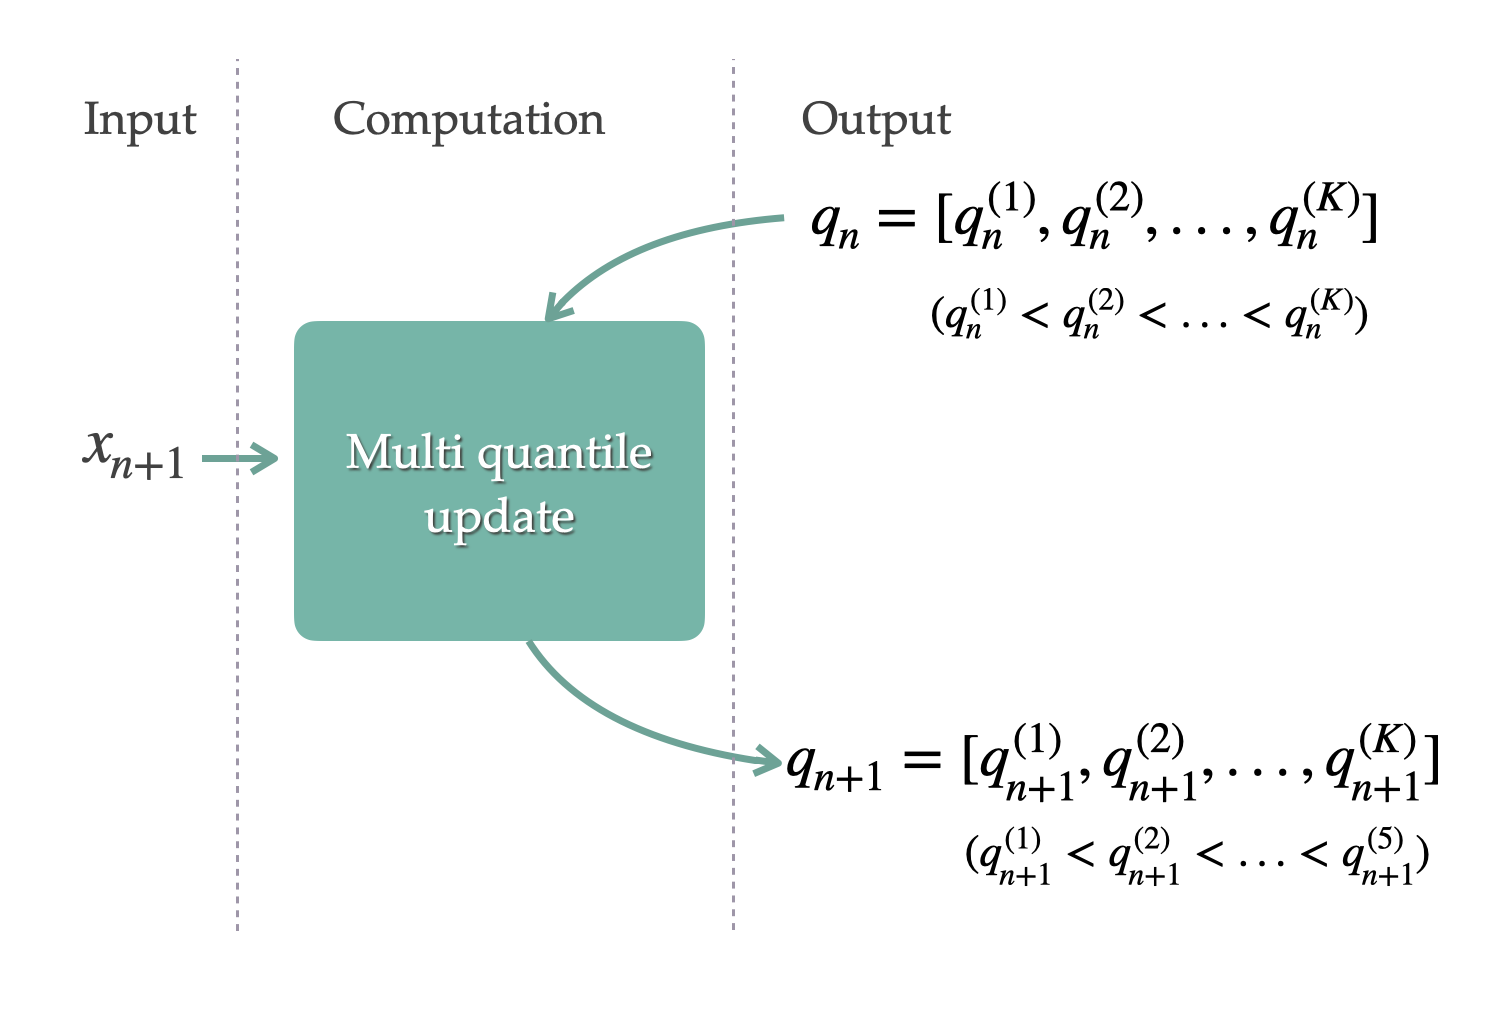
\includegraphics[width=0.7\columnwidth]{Multi_img.png}
	\caption{The update of multi-quantile estimation methods in general}
\end{figure}

A trivial solution for multi-quantile estimation is to run multiple single quantile estimation processes in parallel, such that each quantile is estimated by one process. The multi-process solution however, leads to two main problems:
\begin{enumerate}
    \item The application software/hardware might not have sufficient parallel processing capacity for the algorithm.
    \item Estimating the quantiles independently means the monotone property of quantiles is not taken into account. That is, $\tau_1$-$q > \tau_2$-$q$ if and only if $\tau_1 > \tau_2.$
\end{enumerate}

The following two multi-quantile estimation methods can simultaneously estimate multiple quantile values in one process while utilising the monotonic property. Both algorithms, \textit{shiftQ}\cite{hammerJointTrackingMultiple2019b} and \textit{extended $P^2$}\cite{raatikainenSequentialProcedureSimultaneous1993} utilize the monotone property by ensuring a positive distance between one quantile and its previous quantile, i.e.,
$q_{i} - q_{i-1} > 0$. The shiftQ algorithm is described in section \ref{sec: multi_shiftQ}, and the next section \ref{sec: multi_{p2}} for the extended $P^2$ algorithm.



% ----------------------------------- shiftQ ---------------------------------------

\section{The shiftQ method}
\label{sec: multi_shiftQ}

In general, shiftQ updates its quantile estimates each time a new observation is made. Each update of the algorithm consists of the update of a central quantile followed by updating each other quantile outwards from the center. The central point is updated with the \emph{deterministic update-based multiplicative incremental quantile estimator} (DUMIQE) and the latter are updated using the concept of \emph{shifted distributions}. In this section, we first briefly introduce the DUMIQE algorithm, followed by an explanation of shifted distributions and section \ref{subsec: multi_shiftQ_description} details how the shitQ algorithm uses these concepts to estimate multiple quantile simultaneously.
\\\\
The DUMIQE algorithm updates the quantile estimate upon the arrival of each new observation. It is a development on the work of \citeauthor{tierneySpaceEfficientRecursiveProcedure1983}\cite{tierneySpaceEfficientRecursiveProcedure1983}, which applies a stochastic approximation on quantile estimation. The similarity between DUMIQE and SGD can be seen in the following algorithm pseudo-code:

\begin{algorithm}
    \caption{DUMIQE algorithm}\label{alg:DUMIQE}
    \begin{algorithmic}[1]
        \Require{Data Stream $X$, stepsize $\alpha$}, $\tau$, initial quantile estimate $q_0$ ($q_0 > 0$)
        \Ensure{$q$}
        % \Procedure{frugal}{$X,\tau$}            \Comment{X is the dataset}
        % \State {Initialize} $q$                 \Comment{Requires \textbf{positive initialization} $q$ > 0}
        \State{$q = q_0$}                         \Comment{\textbf{Positive} initialization }
            \For{$x_k$ in $X$}                  \Comment{Parameter update for each input data point}
                % \State \textbf{set} $\alpha_k$  \Comment{Set stepsize}
                \If{$x_k > q$}                  
                    \State{$q = q + \alpha \tau \cdot q$}
                \Else                           
                    \State{$q = q - \alpha (1-\tau)\cdot q$}
                \EndIf
            \EndFor
        \State \textbf{return} $q$              \Comment{$q$ is the DUMIQE estimation result}
    \end{algorithmic}
\end{algorithm}

The update of other quantiles are based on the the relationship with the central quantile. For example, if the central quantile is the median, the $0.25$-quantile is then estimated as the median of distribution below the estimate of median. To apply this idea, DUMIQE uses a shifted distribution $Y$ of the input $X$ such that $X = Y + \delta$, where $\delta$ is the shift constant. In the following method description, we use $Q_X(q)$ and  $Q_Y(q)$ to denote the estimate of $q$ on distribution $X$ and $Y$. In order to distinguish the quantile estimate on different distributions, the DUMIQE algorithm for the $\tau_k$-quantile on distribution $X$ at the observation of the $n$th sample $x_n$ is written as \marginpar{cases to be added to equation}
\begin{align}
        &Q_{X, n+1}(q_k) \leftarrow Q_{X, n}(q_k) + \alpha \tau_k \cdot Q_{X, n}(q_k)  & \text{if } Q_{X, n}(q_k) < x_n \\
        &Q_{X, n+1}(q_k) \leftarrow Q_{X, n}(q_k) - \alpha (1-\tau_k) \cdot Q_{X, n}(q_k)  & \text{if } Q_{X, n}(q_k) \geq x_n \nonumber
\end{align}

\subsection{Method Description}
\label{subsec: multi_shiftQ_description}

\textbf{Motivation}: The difference between the two quantiles for the $x_{n}$ observation is:
$$
diff = |Q_{X,n}(q_{k+1}) - Q_{X,n}(q_k)|
$$
Note that $diff > 0$ for all $x_i, i \in \{1,...,N\}$, so different quantiles never cross each other. This property is guaranteed by the update function DUMIQE() and its restriction that the input quantile estimate must be positive.
\\\\
At the arrival of observation $x_n$, the central quantile estimate $q_c$ is first updated. Denote $K$ as the number of quantiles for estimation. Then the quantile estimates smaller than $q_c$ are updated based on the nearest quantile larger than them, yielding the sequence $\{q_{c-1}, ..., q_1\}$, and conversely the bigger quantile estimates are updated in the order of {$q_{c+1}, ..., q_{K}$}.
\\\\
\textbf{Updating one quantile:} The difference between a quantile $q_{k+1}$ and its neighbour $q_k$ is calculated based on the idea of a "shifted distribution".
Let $X$ denote the original distribution of the data stream, and let the distribution $Y$ denote a shifted version of $X$ such that $Y = X + \delta$ for some constant $\delta$. In this way, the quantile estimate $q_{k+1}$ can be updated by implementation of shifting. The basic steps are:
        \begin{enumerate}
            \item Calculate the shift constant $\delta = Q_{X,n}(q_k)$
            \item Get shifted observation $y_{n,k+1} =  \delta - x_n$ \label{step: shift_observation}
            \item Use the shifted observation to calculate the shifted quantile estimate $Q_{Y, n+1}(q_{k+1})$ with DUMIQE
            \item Shift back to $X$: $Q_{X,n+1}(q_{k+1}) =  \delta  - Q_{Y, n+1}(q_{k+1})$
        \end{enumerate}
When updating a quantile $q_{k-1}$ based on $q_k$, step \ref{step: shift_observation} uses the inverse: $y_{n,k-1} = x_n - \delta$
\\\\
\noindent\textbf{shiftQ update:}
The steps of the shiftQ algorithm are:
\begin{enumerate}
    \item \textbf{Update the central quantile:} Calculate $q_c = Q_{X,n+1}(q_c)$ by DUMIQE 
    \item \textbf{Update the smaller quantiles:} Starting from central quantile $q_c$, the estimates for $q_{c-1}, ..., q_{1}$ are calculated each based on the last.
    \item  \textbf{Update the bigger quantiles:} Similar to step 2, the larger quantiles are estimated for $q_{c+1}, ..., q_{K}$ in sequence.
\end{enumerate}

Pseudocode for the shiftQ algorithm is included as algorithm \ref{alg:multi_shiftQ}.
% \subsection{The shiftQ Algorithm}
\begin{algorithm}
    \caption{The shiftQ Algorithm}\label{alg:multi_shiftQ}
        \begin{algorithmic}[1]
            \Require
            \State{Dataset $X$ (with positive data points only)}
            \State{Target quantile values $[\tau_1, \tau_2, ..., \tau_K]$}
            \State{Central position $c$, Number of quantiles $K$}
            \State{Stepsize $\alpha_X$, Stepsize $\alpha_Y$}
            \State{Quantile Estimate Initialization on $X$: {$0 < Q_{X,0}(q_1) < ... < Q_{X,0}(q_K)$}}
            \State{Quantile Estimate Initialization on $Y$: {$0 < Q_{Y,0}(q_1) < ... < Q_{Y,0}(q_K)$}}
            \Ensure{Target quantile estimates $[\tau_1\text{-}q, \tau_2\text{-}q, ..., \tau_K\text{-}q]$}

            \State
            \State{Choose some $c \in {1,..K}$, usually the middle point}
            \State{$q_c \gets Q_{X,0}(q_c)$}
            \For{$x_n \in X$}
                \LineComment{Update central quantile}
                \State{$q_c \leftarrow DUMIQE(q_c, x_n, \tau_c, \alpha_X)$}
                \State{}

                \For{$k \in \{c-1, ..., 1\}$}
                \LineComment{Update smaller quantiles}
                    \State{$\delta \leftarrow Q_{X,n+1}(q_{k+1})$}
                    \State{$y_{n,k+1} \leftarrow Q_{X,n}(q_{k+1}) - x_n$}
                    \State{$Q_{Y, n+1}(q_{k}) \leftarrow DUMIQE(Q_{Y, n}(q_{k}), y_{n,k+1}, q_k, \alpha_Y)$}
                    \State{$Q_{X,n+1}(q_{k}) \leftarrow \delta - Q_{Y, n+1}(q_{k+1})$}
                \EndFor
                \State{}

                \For{$k \in \{c+1, ..., K\}$}
                \LineComment{Update bigger quantiles}
                    \State{$\delta \leftarrow Q_{X,n+1}(q_{k-1})$}
                    \State{$y_{n,k-1} \leftarrow  x_n - Q_{X,n}(q_{k-1})$}
                    \State{$Q_{Y, n+1}(q_{k}) \leftarrow DUMIQE(Q_{Y, n}(q_{k}), y_{n,k-1}, q_k, \alpha_Y)$}
                    \State{$Q_{X,n+1}(q_{k}) \leftarrow \delta + Q_{Y, n+1}(q_{k-1})$}
                \EndFor
            \EndFor

            \State
            \LineComment{Return final estimaton}
            \State{$[\tau_1\text{-}q, \tau_2\text{-}q, ..., \tau_K\text{-}q] \leftarrow [Q_{X,N}(q_1), ..., Q_{X,N}(q_K) ]$}
        \end{algorithmic}
\end{algorithm}
\subsection{Experiment Results}

There are two experiments run on shiftQ algorithm. Refer to \textcolor{blue}{insert chapter reference here} for the details of the experiment settings. The first one aims to compare the quantile crossing behaviour of shiftQ and SGD, and the second one tests shiftQ's performance on quantile estimation.

In the first experiment, the experiment dataset is 5000 samples generated from a uniform distribution over the range $(0,100)$. All data points are required to be positive as the prerequisite of the shiftQ algorithm. This experiment compares two algorithms, shiftQ and SGD, and examines the quantile crossing behaviour of each algorithm.

\marginpar{Fig \ref{fig: shiftQ_SGD} graphic needs axis labels}
\begin{figure}[h!]
	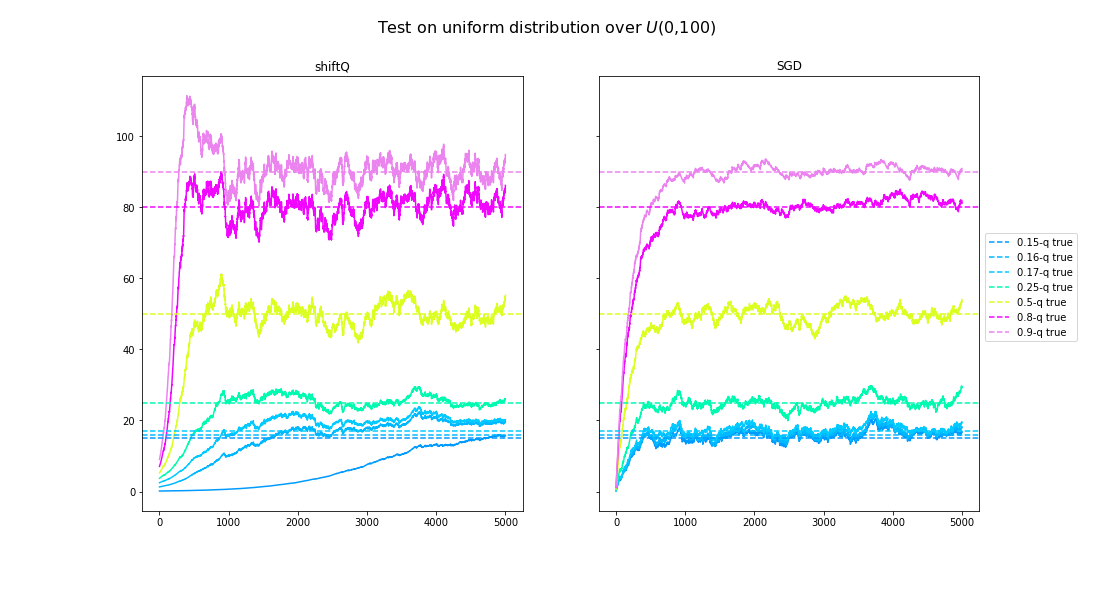
\includegraphics[width=1\columnwidth]{shiftQ/shiftQ_vs_SGD.png}
    \caption{Two process plots comparing the estimation of quantiles 0.15-q, 0.16-q, 0.17-q, 0.25-q, 0.8-q and 0.9-q with shiftQ and SGD over a uniform distribution.}
    \label{fig: shiftQ_SGD}
\end{figure}

\marginpar{``epoch'' terminology under review}
Figure \ref{fig: shiftQ_SGD} shows the estimates by shiftQ and SGD over 5000 epochs in the first experiment. In this experiment, $0$ crossings occurred in the shiftQ implementation, while SGD caused 33 crossings. Over 100 repetitions of this experiment, the average number of crossings by SGD is 72.48, with a standard deviation of 66.23. The crossings in SGD have two interesting properties:
    \begin{enumerate}
        \item The crossings are likely to occur when two quantile values are close to each other. For example, in this example, only two pairs of quantiles ($0.15$, $0.16$) and ($0.16$, $0.17$) are detected to have crossings. The difference between the true quantile values of these pairs is 1, while the other adjacent quantile pairs are at least 8 away from each other. Given the stepsize was set to $\alpha = 0.45$ for SGD, the short distance between two adjacent quantile values are likely to be the main cause of crossings.
        \item The crossings happen are likely to happen in a slot of concentrated continuous epochs. For example, among the 33 crossings, 11 of them are between $0.16$-q and $0.17$-q from epoch 2400 to 2410. The other 22 crossings are between $0.15$-q and $0.16$-q continuously from epoch 3489 to 3510. This suggests that once a crossing takes place, its impact is likely to continue for the following epochs until the crossing is fixed.
    \end{enumerate}

The second experiment aims to investigate the effectiveness of shiftQ algorithm. Figures \ref{fig: shiftQ_proc}, \ref{fig: shiftQ_res} and \ref{fig: shiftQ_err} show process plots for the shiftQ algorithm run on the absolute value of 1000 samples from \textit{gau-1}.

\begin{figure}[h!]
	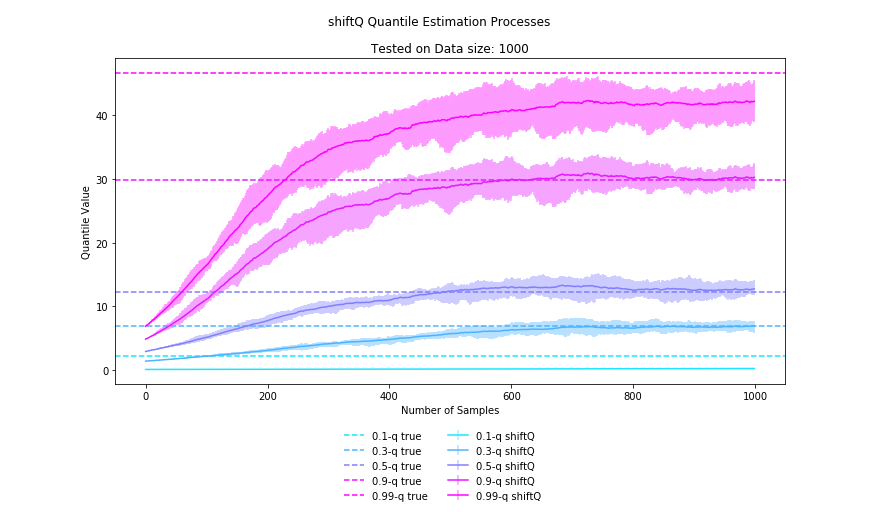
\includegraphics[width=1\columnwidth]{shiftQ/1000_proc.png}
	\caption{The shiftQ algorithm for Positive Gaussian 1 distribution (the process graph)}
    \label{fig: shiftQ_proc}
\end{figure}

\begin{figure}[h!]
	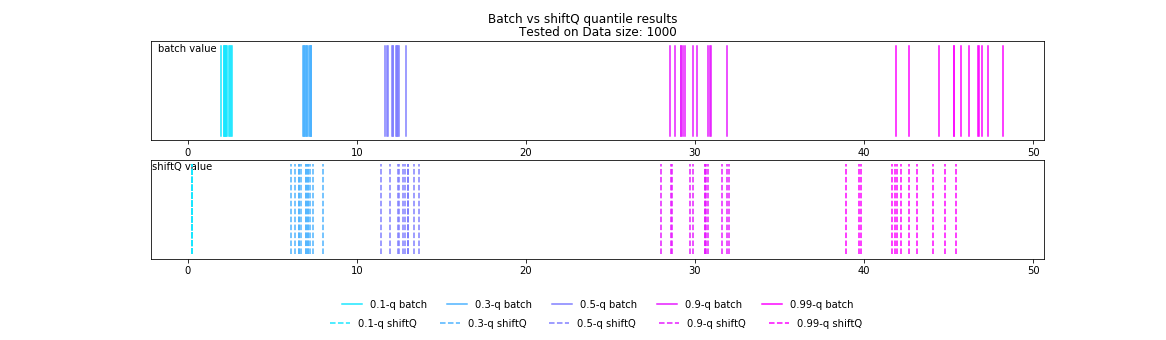
\includegraphics[width=1\columnwidth]{shiftQ/1000_res.png}
	\caption{The shiftQ algorithm for Positive Gaussian 1 distribution (the result graph)}
    \label{fig: shiftQ_res}
\end{figure}

\begin{figure}[h!]
	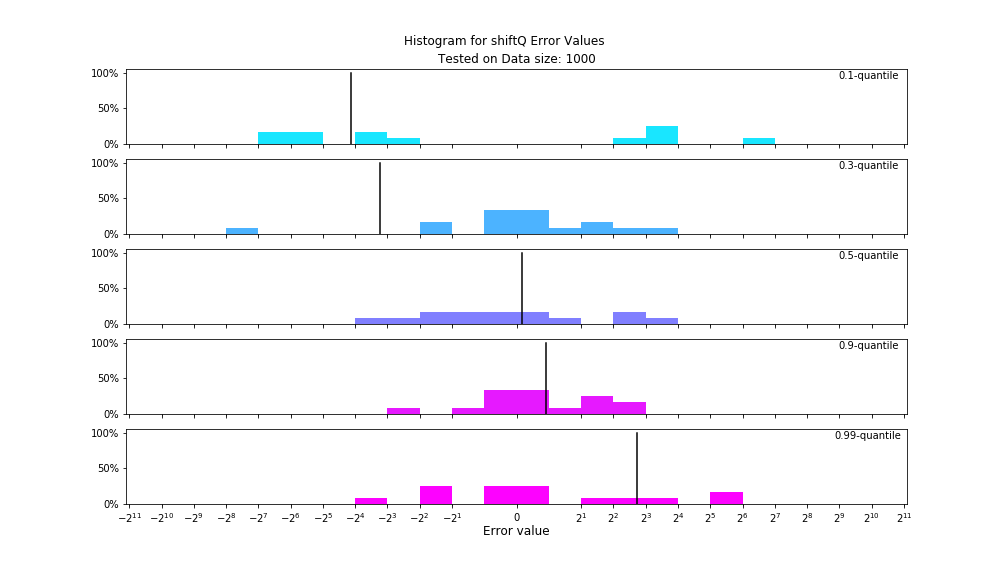
\includegraphics[width=1\columnwidth]{shiftQ/1000_err.png}
	\caption{The shiftQ algorithm for Positive Gaussian 1 distribution (the error graph)}
    \label{fig: shiftQ_err}
\end{figure}

\begin{figure}[h!]
	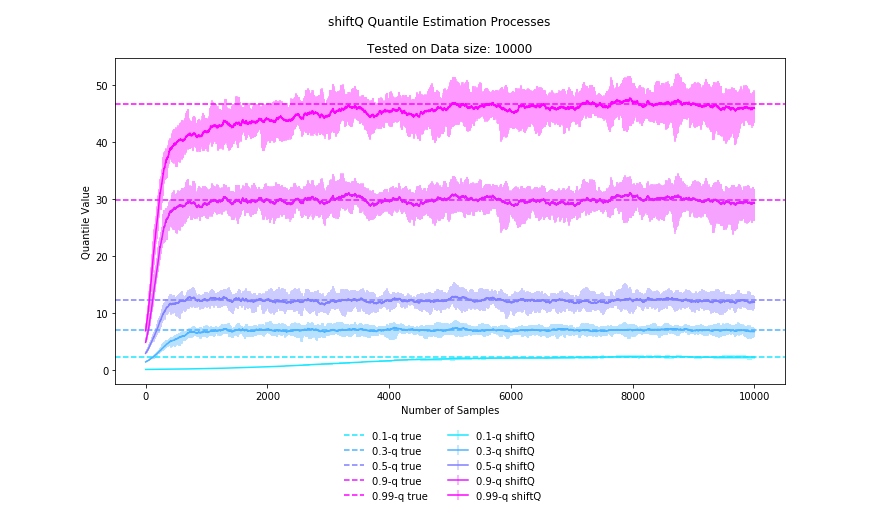
\includegraphics[width=1\columnwidth]{shiftQ/10000_proc.png}
	\caption{The shiftQ algorithm for Positive Gaussian 1 distribution (the process graph)}
    \label{fig: shiftQ_proc_10000}
\end{figure}

 In the process plot in Fig \ref{fig: shiftQ_proc} the quantile estimates for $0.1$-q and $0.99$-q have not converged even after 1000 epochs. From the comparison with the 0.5-q we can see that this big error is not caused by the initialization value of 0.1-q. Specifically, the shiftQ 0.5-q converges even though the true quantile of it is further away from its initialization. Instead, the estimation of 0.1-q has barely changed during the 1000 epochs. The converging trend of 0.99-q is also too slow to reach the true 0.99-q quantile within 1000 epochs. The distance between the batch quantiles and shiftQ estimated quantiles in Fig \ref{fig: shiftQ_res} has shown that the quantile estimates at both ends are far away from the batch quantiles. It is shown in the Fig \ref{fig: shiftQ_err} that the shiftQ algorithm has a largely varied performance on different quantiles. For example, the 0.5 and 0.9 quantiles has a much smaller and stable error distribution around 0, while the 0.1 quantile has a wide range of error values from less than -100 to more than 50. 
 
 To test the convergence of end quantile values, a further experiment is done with a dataset of 10000 samples. Fig \ref{fig: shiftQ_proc_10000} shows that both 0.1-q and 0.99-q estimates finally converge when there are a sufficient amount of samples.
% ----------------------------------- Extended P2 ---------------------------------------
\pagebreak
\section{The Extended $P^2$ Algorithm}
\label{sec: multi_{p2}}

The \textit{Extended $P^2$} algorithm\cite{raatikainenSequentialProcedureSimultaneous1993} uses exactly the same idea as the $P^2$ algorithm\cite{jainP2AlgorithmDynamic1985}. So for a better understanding, we introduce the $P^2$ algorithm first in \ref{subsubsec: description_{p2}}, then the generation method for the extended $P^2$ algorithm.
In section \ref{subsec: algo_extended_{p2}}, the detailed algorithm for extended $P^2$ is provided, followed by its experiment results in section \ref{subsec: exp_extended_{p2}}.

\subsection{Method Description}
\subsubsection{The $P^2$ Method}
\label{subsubsec: description_{p2}}

The intuition of the $P^2$ method is the assumption that any three adjacent quantiles form a parabolic formula.
Specifically, the method interprets quantile estimation as a relationship based on quantile values and their ordering positions, and applies either linear or parabolic adjustments based on the information from their neighbours.

Consider the straightforward quantile computation for [$\tau_1, ..., \tau_K$] that sorts all observations from the dataset $X = \{x_i\}^N_1$. Let $x_i$ denote the $i$th smallest value of $X$, then we have $x_1 < x_2 < ... < x_N$. 
To find the $\tau_i$-quantile of $X$, we need to find the data observation at \textit{marker position} $m_i = \tau_i (N-1) + 1$. Given the marker position, we then retrieve the value of the marker, the corresponding \textit{quantile value} $q_i = x_{m_i}$. 
For 3 adjacent quantiles at $\tau_{i-1}, \tau_i, \tau_{i+1}$, their quantile values can be independently computed in the same way, as shown in Figure \ref{fig: {multi_relationship_p2}}.

\begin{figure}[h]
    \centering
	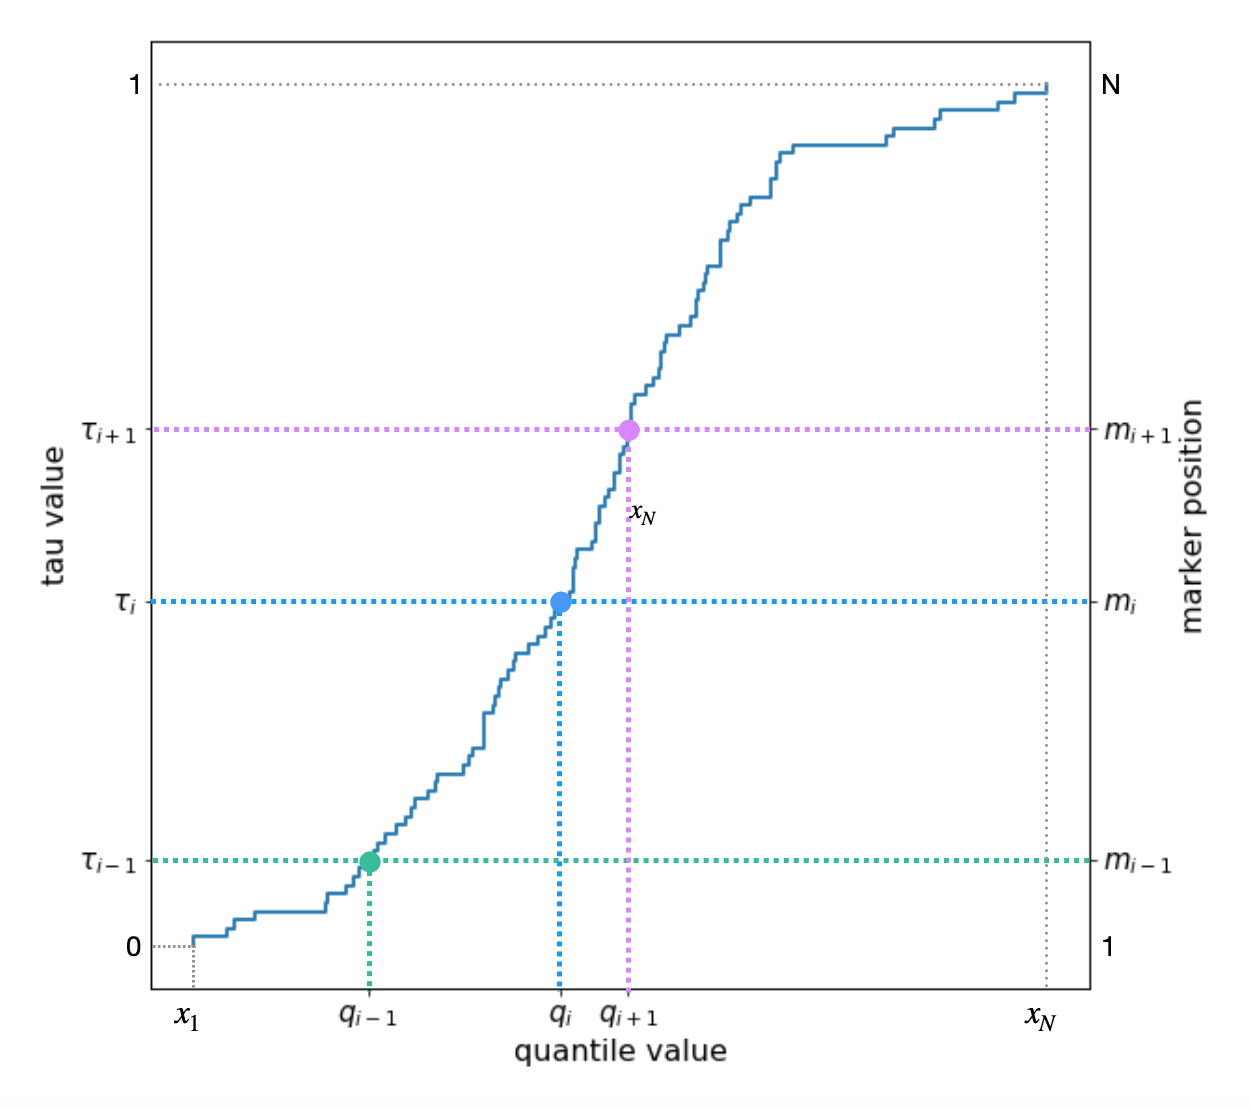
\includegraphics[width=0.8\columnwidth]{P2/relationships.png}
    \caption{Relationship between $\tau$ value, marker position and quantile values correspondingly for 3 adjacent quantiles}
    \label{fig: {multi_relationship_p2}}
\end{figure}

For quantile estimation, however, storing and sorting the entire dataset is infeasible. The $P^2$ method records only information only about the Target quantile values, and update them on the arrival of new observations. The update method, based on different conditions, is either a \textit{Piecewise-Parabolic} ($P^2$) formula, or a linear formula.

The information recorded for the $i$th quantile contains 3 parts: the marker position $m_i$, the desired marker position $m_i^\prime$, and the quantile value $q_i$. For quantile $\tau_i$ with current observation number $N$, the desired marker position is $m_i^\prime = 1 + (N-1)\tau$. This algorithm aims to keep each marker position $m_i$ close to its desired position $m_i^\prime$ as new observation come in. As $m_i$ is updated, $q_i$ is updated to an estimate of the new value of the $m_i$th data point.
% The quantile value estimation $q_i$ is then updated accordingly after the current marker position is fixed.
Figure \ref{fig: {multi_parabolic_p2}} demonstrates the update of $m_i$ and $q_i$.

\begin{figure}[h]
    \centering
	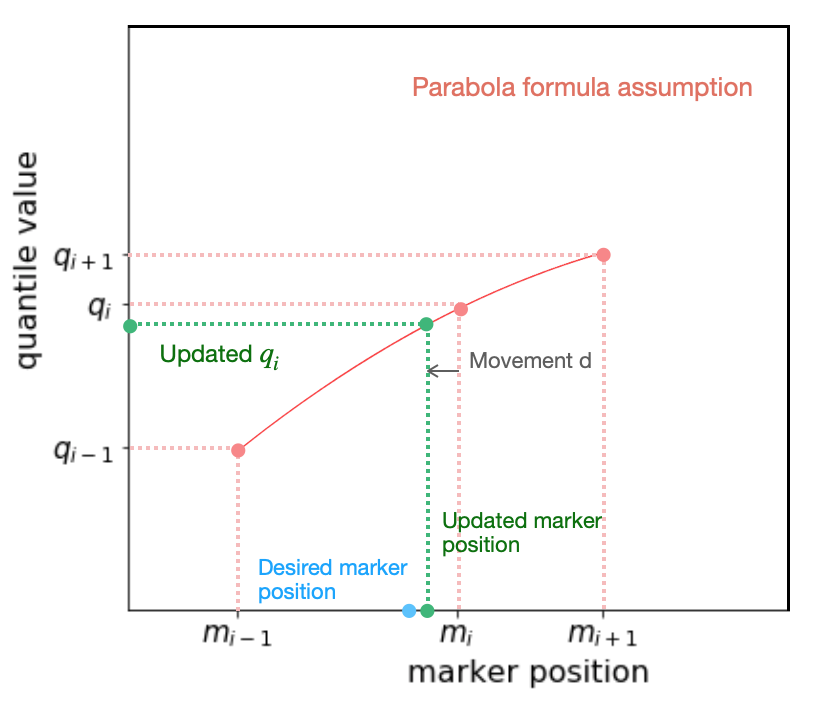
\includegraphics[width=0.7\columnwidth]{P2/parabola.png}
    \caption{Quantile value update using the Piecewise-Parabolic($P^2$) formula}
    \label{fig: {multi_parabolic_p2}}
\end{figure}

The quantile value update is based on the Piecewise-Parabolic assumption that any three adjacent makers form a parabolic curve of the form $q_i = aq_i^2 + bq_i + c$.

If a marker is moved $d$ positions to the right, the new quantile value is updated by the \textit{parabolic formula}:
\begin{align}
\begin{split}
    q_{i} \leftarrow q_{i}+ & \frac{d}{m_{i+1}-m_{i-1}}\\
    \cdot & { \bigg[ 
        \left(m_{i}-m_{i-1}+d\right) \frac{\left(q_{i+1}-q_{i}\right)}{\left(m_{i+1}-m_{i}\right)}
        +\left(m_{i+1}-m_{i}-d\right) \frac{\left(q_{i}-q_{i-1}\right)}{\left(m_{i}-m_{i-1}\right)}
        } \bigg] \\
    m_{i} \leftarrow m_{i}+&d \text{ where } d = \pm 1
\end{split}
\end{align}

When applying the parabolic update would violate the monotone property, the alternative update is a \textit{piecewise-linear formula}:
\begin{equation}
    \begin{array}{l}
    q_{i}=q_{i}+d \frac{\left(q_{i+d}-q_{i}\right)}{m_{i+d}-m_{i}} \\
    m_{i}=m_{i}+d
    \end{array}
\end{equation}

In short, the update method for $\tau_i$-quantile takes only 2 steps:\\
Before starting, the $P^2$ algorithm extends the set of target quantiles $\tau_1 <... < \tau_K$ with $0$ and $1$, giving the target quantiles $[0, \tau_1, ..., \tau_K, 1]$.
When a new observation comes,
\begin{enumerate}
    \item Update every marker position $m_i$ to approach the desired marker position $m_i^\prime$.
    \begin{enumerate}
        \item If the quantile value is bigger than the coming observation, move the marker position by one position to the right.
        \item Adjust the marker position again if it is more than one position away from the desired marker. The move $d$ is $1$ if the marker position moves right, and $-1$ for moving left.
    \end{enumerate}
    \item Update the quantile value
    \begin{enumerate}
        \item Try applying the parabolic update to the quantile value. Note it might change the increasing order of quantiles, that is, $q_{i+1} > q_{i}$.
        \item If the ordering of quantile values is changed by the parabolic update, try the linear update instead.
    \end{enumerate}
\end{enumerate}


\subsubsection{The Extended $P^2$ Method}
In $P^2$, the update of a quantile relies on its position relative to the neighbour markers, indicating the accuracy of neighbour marker positions is important. 
It sets one marker for each quantile value, that is, a total of $K$ markers for [$\tau_1, ..., \tau_K$].
The extended $P^2$ algorithm improves the estimation accuracy by the introduction of "middle markers",  which nearly doubles the amount of markers in $P^2$. 
This means, in the initialization part, there will be $2K+3$ markers for
$$
\tau = 0, \frac{0+\tau_1}{2}, \tau_1, \frac{\tau_1 + \tau_2}{2}, \tau_2, ..., \tau_{K}, \frac{\tau_K+1}{2}, 1
$$
And the estimation update for all those markers follows the same rule as in the $P^2$ algorithm.

The only difference between extended $P^2$ and $P^2$ is the extension of markers at the initialization stage. At a doubly expensive computation cost, the quantile estimation reaches a higher accuracy from the extra information, as shown in the work of \citeauthor{raatikainenSequentialProcedureSimultaneous1993}\cite{raatikainenSequentialProcedureSimultaneous1993}. Besides the extra information brought by the extra markers, the extended $P^2$ algorithm also benefits from a better initialization by a larger sampling. The larger sampling in extended $P^2$ reduces the possibility of severely unevenly distributed initializations, which becomes important for  $P^2$, as it is sensitive to the initialization of quantiles.
% In $p^2$, only desired quantiles have their information recorded and used for 

% \subsection{The Algorithm of Extended $P^2$}
% \label{subsec: algo_extended_{p2}}
Pseudocode for the $P^2$ algorithm is presented in algorithm \ref{alg:multi_p2} followed by the extended $P^2$ algorithm in algorithm \ref{alg:multi_ext_p2}.
\begin{algorithm}
    \caption{The $P^2$ Algorithm}\label{alg:multi_p2}
        \begin{algorithmic}[1]
            \Require{Dataset $X$, $K$ target quantile values $[\tau_1, \tau_2, ..., \tau_K]$}
            \Ensure{Targe quantile estimates $[\tau_1\text{-}q, \tau_2\text{-}q, ..., \tau_K\text{-}q]$}
            \State
            \State {\textbf{0.Extend number of markers from $K$ to $K' = K+2$}}
            \LineComment{Add $0$ and $1$ before and after the target quantiles.}
            \State{$[\tau_1^\prime, \tau_2^\prime, ..., \tau_{K'}^\prime] = [0, \tau_1, \tau_2, ..., \tau_{K}, 1]$}
            \State
            \State{\textbf{A. Initialization}}
            \State {The first $K'$ observations (sorted): \{$x_1,x_2,...,x_{K'}$\}}
            \For{$(i = 1, ..., K')$}
                \State {Marker height:    $q_i = x_i $}
                \State {Marker position:   $m_i = i$}
                \State {Desired Marker position:  $m_i^\prime = ((K')-1)\tau_i + 1$}
            \EndFor

            \State
            \State{\textbf{B. For each new observation $x_j$, $j \geq K'+1$, perform the following}}
            \Switch{$s$}            \Comment {Find the cell $k$ such that $q_k \leq x_j < q_{k+1}$}
                \Case{$x_j < q_1$}
                    \State{$q_1 = x_j, k = 1$}
                \EndCase
                \Case{$q_i \leq x_j < q_{i+1}$}
                    \State {$k = i$}
                \EndCase
                \Case{$q_K < x_j$}
                    \State {$q_K = x_j, k = K'-1$}
                \EndCase
            \EndSwitch
            \State
            
            \State{$m_i = m_i + 1$; $i = k+1, ..., K'$}       \Comment{Increment markers above new observation}
            % \Comment{Different from that on the $P^2$ paper}
            \State{$m_i^\prime = m_i^\prime + \tau_i'$; $i = 1, ..., K'$}            \Comment{Update all the desired positions}

            \State
            \State{Adjust marker heights $2$ to $K'-1$ if necessary:}
            \For{$i = 2, 3, ..., K-1$}
                \State {$d_i = m_i^\prime - m_i$}
                \If {($ d_i \geq 1 \text{ and }  m_{i+1} - m_i > 1$) or 
                     ($ d_i \leq -1 \text{ and }  m_{i-1} - m_i < -1$) }
                    \State {$d_i = sign(d_i)$}
                    \State {$q_i^\prime = \text{parabolic}(q_i)$}     \Comment{Try the $P^2$ update}
                    \If {$ q_{i-1} < q_i^\prime < q_{i+1}$}
                        \State {$q_i = q_i^\prime$}
                        \Else                           \Comment{Else use linear update}
                            \State{$q_i = \text{linear}(q_i)$}
                    \EndIf
                    \State {$m_i = m_i + d_i$}          \Comment{Update marker position}
                \EndIf
            \EndFor

            \State
            \State {\textbf{C. Return quantile estimates} }     
            \LineComment{The result is available after any number of observations}
            \State {$[\tau_1\text{-}q, \tau_2\text{-}q, ..., \tau_K\text{-}q] = [q_2, q_2, ..., q_{K+1}]$}
        \end{algorithmic}
\end{algorithm}
\\\\
The extended $P^2$ extends the number of quantile markers of the $P^2$ algorithm at the initialization step, then follows $P^2$ in the next steps.

\begin{algorithm}
    \caption{Extended $P^2$ Algorithm}\label{alg:multi_ext_p2}
        \begin{algorithmic}[1]
            \Require{Dataset $X$, Demanding quantile values $[\tau_1, \tau_2, ..., \tau_K]$}
            \Ensure{Demaning quantile estimates $[\tau_1\text{-}q, \tau_2\text{-}q, ..., \tau_K\text{-}q]$}

            \State
            \State {\textbf{0.Extend number of markers from $K$ to $2K+3$}}
            \LineComment{Evenly fill the intervals between $0,1$ and each 2 quantile values}
            \State{$[\tau_1^\prime, \tau_2^\prime, ..., \tau_{2K+3} ^\prime] = [0, \frac{0+\tau_1}{2}, \tau_1, \frac{\tau_1 + \tau_2}{2}, \tau_2, ..., \tau_{K}, \frac{\tau_K+1}{2}, 1]$}

            \State
            \State{\textbf{1. Apply $P^2$ with the extended initialization}}
            \LineComment{And returns an estimate of extended list}
            \State{$[q_1^\prime, ..., q_{2K+3}^\prime] = P^2$ ($X$, $[\tau_1^\prime, \tau_2^\prime, ..., \tau_{2K+3} ^\prime]$)}
            \State
            \State {\textbf{2. Return quantile estimates} } 
            \State {Extract the quantile estimates for the original $M$ quantile values}
            \State {$[\tau_1\text{-}q, \tau_2\text{-}q, ..., \tau_K\text{-}q] = [q_3^\prime, q_5^\prime, ..., q_{2K+1}^\prime]$}
        \end{algorithmic}
\end{algorithm}

% 0, 0.5, 1, 1.5, 2, ..., M,    (M+1)/2, 1
% 1, 2,   3, 4,   5, ..., 2M+1, 2M+2,   2K+3            

\subsection{Experiment Results}
\label{subsec: exp_extended_{p2}}
The $P^2$ algorithm is tested on the Gaussian 1 distribution on 1000 samples.The process plot Fig \ref{fig: p2_proc} shows the convergence of different quantiles have slightly different pace, in that the 0.9 and 0.99 are very close to the true quantile value while the other 3 have already stayed stable at the 1000th epoch. Fig \ref{fig: p2_res} shows the final results are close, which is evaluated in Fig \ref{fig: p2_err} that error values of extended $p^2$ estimates has limited error values between -20 and 10 for all quantiles except for one outlier at -80. 
Overall the extended $P^2$ method has a really fast convergence rate.

\begin{figure}[h!]
	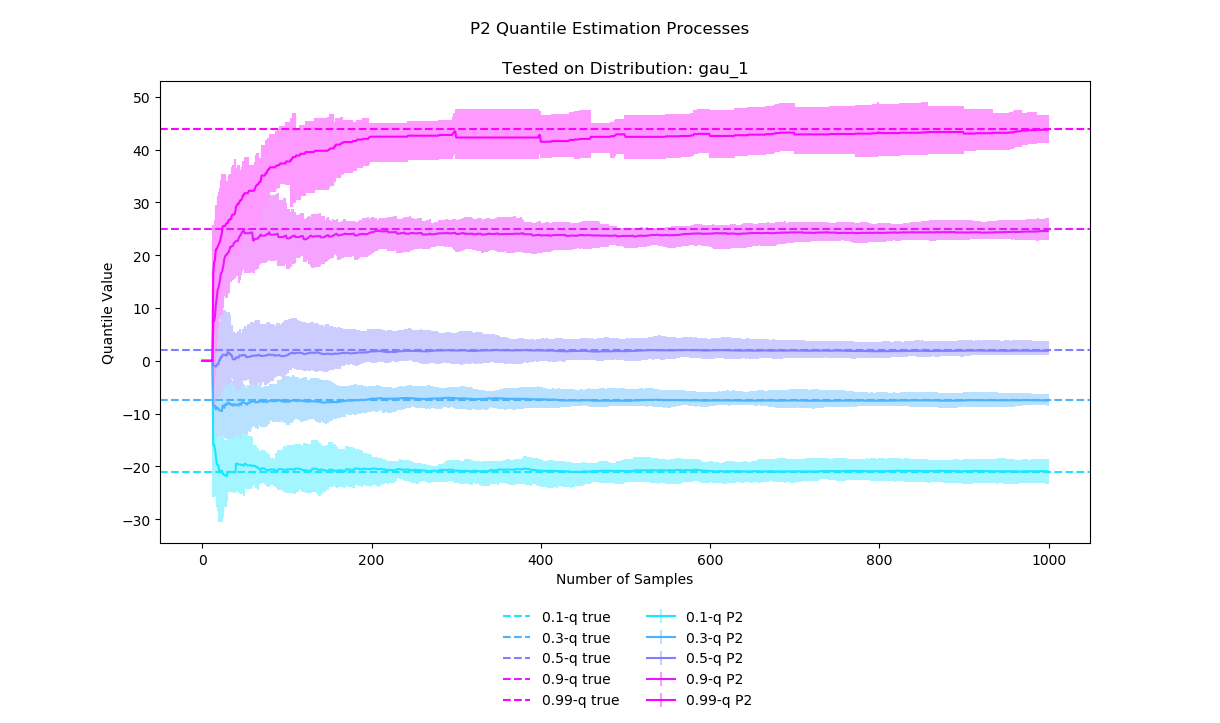
\includegraphics[width=1\columnwidth]{P2/gau_1_proc.png}
    \caption{The extended $P^2$ algorithm for Gaussian 1 distribution (the process graph)}
    \label{fig: p2_proc}
\end{figure}

\begin{figure}[h!]
	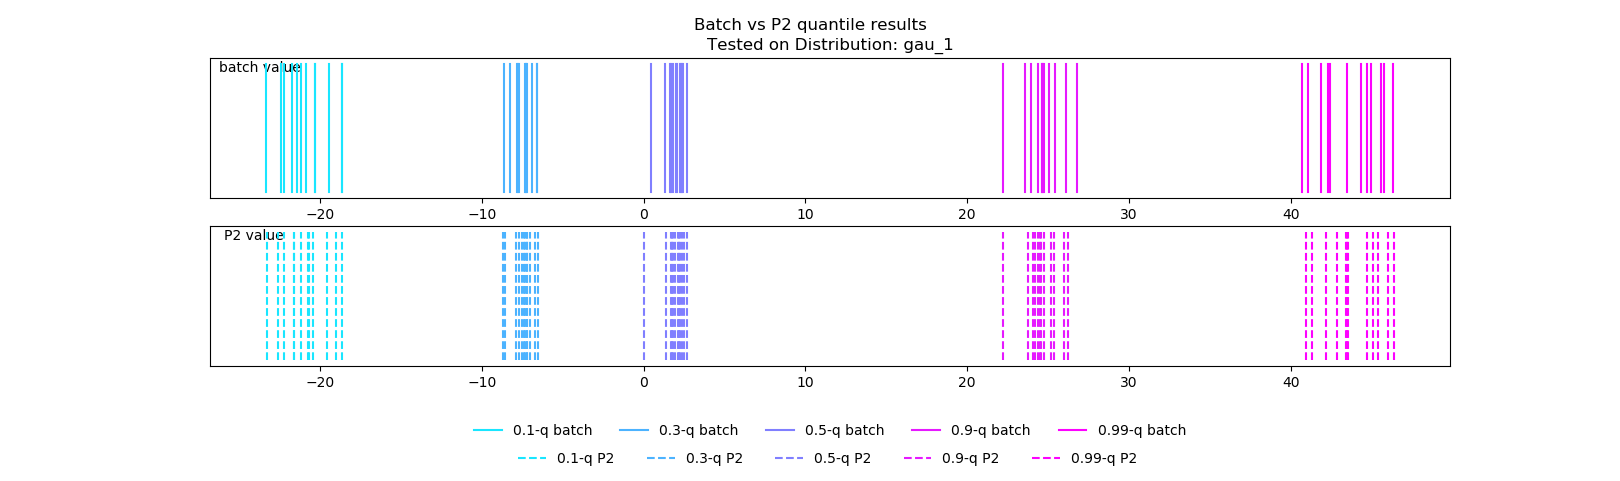
\includegraphics[width=1\columnwidth]{P2/gau_1_res.png}
	\caption{The extended $P^2$ algorithm for Gaussian 1 distribution (the result graph)}
    \label{fig: p2_res}
\end{figure}

\begin{figure}[h!]
	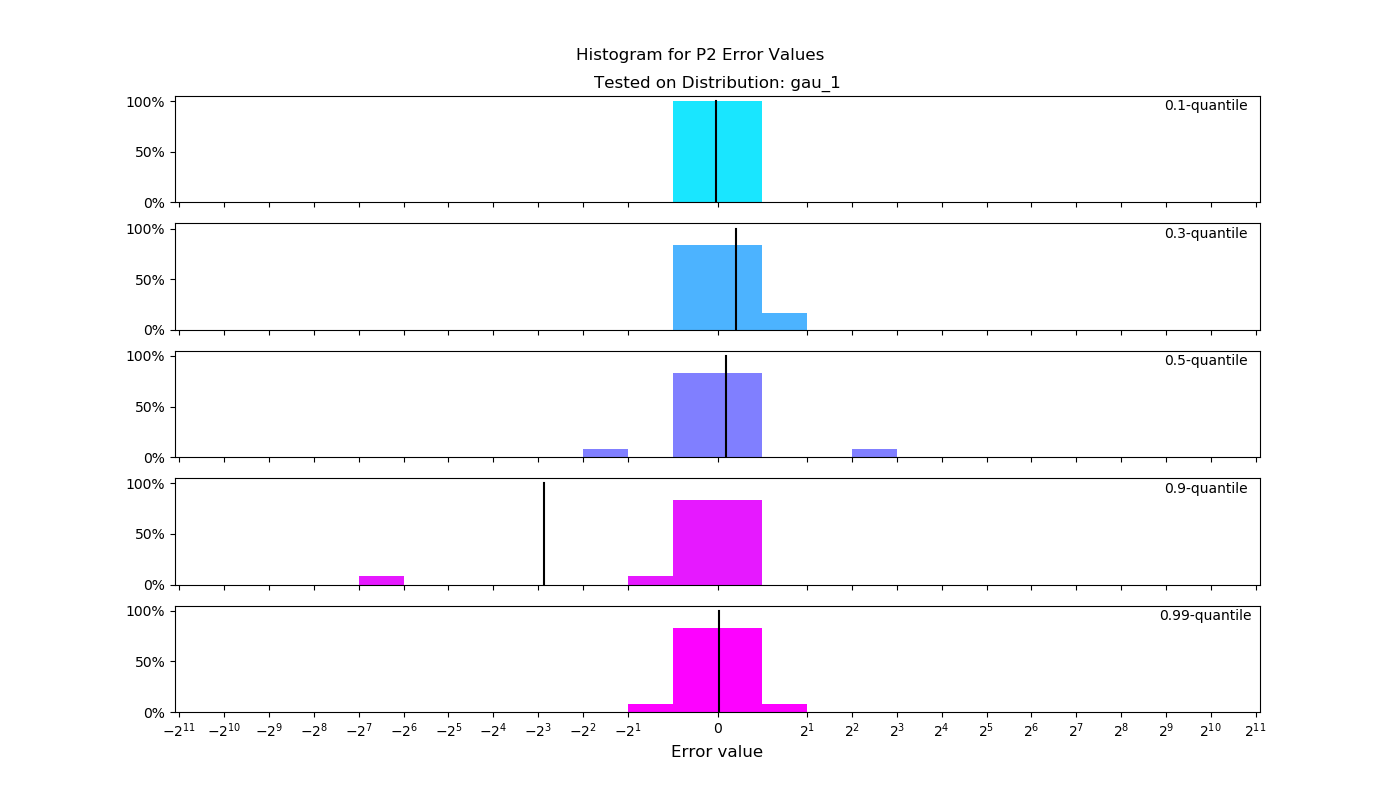
\includegraphics[width=1\columnwidth]{P2/gau_1_err.png}
    \caption{The extended $P^2$ algorithm for Gaussian 1 distribution (the error graph)}
    \label{fig: p2_err}
\end{figure}

\marginpar{this will be edited later}
\section{Discussion}
\marginpar{why extended p2 better than shiftQ}
\begin{enumerate}
    \item  P2 has a better initialization point of quantiles, while the initialization of shiftQ is very random. The initialization of quantile estimation methods are very important.
    \item shiftQ is sensitive to its initialization of the relative position between original distribution $Q_X$ and shifted distribution $Q_Y$, which makes is double messy.
    \item Extra information from extended p2: 2K+3 quantiles are used, instead of only K
    \item The mechanism of extended P2 is to insert every new observation into an interval between corresponding markers, which is pretty accurate. shiftQ, however, do not even have a correct update function (should've been the pinball loss function)
\end{enumerate}

\section{Conclusion}
\label{sec: multi_discussion}

\marginpar{to be finished}
From the experimental results we can see the two multi-quantile estimation methods can solve the crossing problem by introducing some mathematical relationship assumptions between adjacent quantiles. The following step will be doing nothing but to 